%%%%%%%%%%%%%%%%%%%%%%%%%%%%%%%%%%%%%%%%%%%%%%%%%%%%%%%%%%%%%%%%%%%%%%%%%%%%%%%%
%2345678901234567890123456789012345678901234567890123456789012345678901234567890
%        1         2         3         4         5         6         7         8

\documentclass[a4paper, 10pt, conference]{ieeeconf} 
\usepackage{graphicx}
\title{\LARGE \bf
Visualization module solving logical problems for the FORMULA system
}


\author{Ksenia Panova% <-this % stops a space
}


\begin{document}

\maketitle
\thispagestyle{empty}
\pagestyle{empty}



%%%%%%%%%%%%%%%%%%%%%%%%%%%%%%%%%%%%%%%%%%%%%%%%%%%%%%%%%%%%%%%%%%%%%%%%%%%%%%%%
%\begin{abstract}
%\end{abstract}


%%%%%%%%%%%%%%%%%%%%%%%%%%%%%%%%%%%%%%%%%%%%%%%%%%%%%%%%%%%%%%%%%%%%%%%%%%%%%%%%
\section{INTRODUCTION}

We have designed the module of visualization of solutions obtained via the smt solver Formula. Solvers for satisfiability modulo theories (SMT) check the satisfiability of first-order formulas containing operations from various theories such as the booleans, bit-vectors, arithmetic. A thorough consideration of various methods of visualization was made. As a result of studies the declarative programming language for solutions of logic problems such as Einstein task or the problem of queens was developed.

\section{PROBLEMS}
The developed system is designed for data visualization. The purpose of the study is to consider an information visualization solutions of logical problems derived from the FORMULA system, which is fundamentally different from existing visualization tools. The most obvious advantage of the new system is that the developed module operates with a much smaller amount of information, which saves time and expense of resources for the visualization process.\\
The main task of the investigation is to design an integrated module of visualization solutions and the results of logical tasks.\\
The developed module should maintain the following functions:
\begin{enumerate}
\item Integration module logical solution FORMULA tasks, analysis of the results of using it
\item Display of static solutions with support for the following types of visualization:
\begin{enumerate}
\item Table
\item Counts
\item Vectors
\end{enumerate}
\item Display of the process of solving problems by means of a dynamic visualization:
\begin{enumerate}
\item Moving objects
\item Time Management
\end{enumerate}
\end{enumerate}

\section{ARCHITECTURE DESIGN}

The project structure is shown in Fig.~\ref{fig:structure}
The system is a program running in Windows. It analyzes configured via FORMULA file, and loads the content to the respective variable depending on the type of task and the format:
\begin{itemize}
\item For a static display in a table - table
\item For dynamic display - sequence
\end{itemize}
\begin{figure}[h]
    \centering
    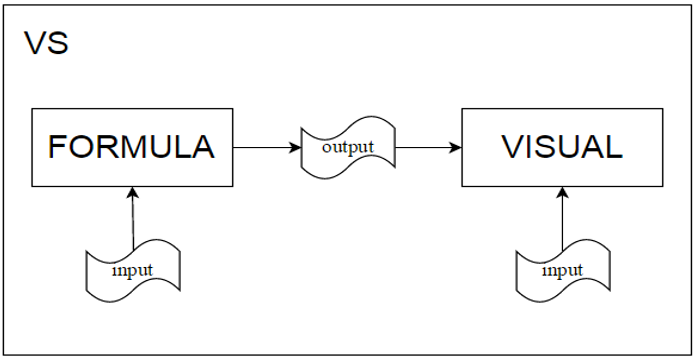
\includegraphics[width=0.4\textwidth]{structure.png}
    \caption{Project structure}
    \label{fig:structure}
\end{figure}


\section{LANGUAGE MODULE}
Starting the system designed by the programming language is accompanied by its conversion into a form that is meaningful to the computer. Therefore, we need a program that reads the text written in one language (the source) and translates it into an equivalent text in another language.\\
In order to provide this, compiler that converts a program written in the language of visualization, in a program written in C ++ was developed.\\
For that, lexer performs lexical analysis which is the process of converting a sequence of characters  into a sequence of tokens (strings with an identified "meaning"). Lexical analysis was performed using parser generator "Lex".\\
After lexical analysis is the syntactic analysis. Parsing or syntactic analysis is the process of analysing a string of symbols, either in natural language or in computer languages, conforming to the rules of a formal grammar. The purpose of syntactic analysis is to determine the structure of the input text. This structure consists of a hierarchy of phrases, the smallest of which are the basic symbols and the largest of which is the sentence. The structure can be described by a tree with one node for each phrase. Basic symbols are represented by values stored at the nodes. The root of the tree represents the sentence. an example is shown in Fig.~\ref{fig:parsetree}. Syntactic analysis was performed using generator "Yacc", which provides automatic construction of grammatical analysis procedures.\\
As a result of the joint compilation of the generated lexer and parser , executable file visual.exe is created for handling of code with new syntax.
\begin{figure}[h]
    \centering
    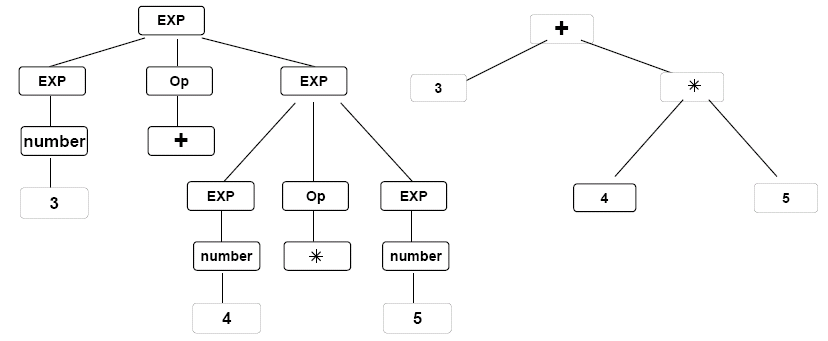
\includegraphics[width=0.5\textwidth]{parsetree.png}
    \caption{Example of syntactic analysis}
    \label{fig:parsetree}
\end{figure}

\section{CONCLUSIONS}

As a result of studies the integrated module of visualization solutions and the results of logical tasks was designed. Also visualization language was developed. For that rules and  a new programming language syntax  have been formulated, on the basis of which carried out the lexical, syntactic and semantic analysis. Graphical system module is also designed to visualize input data in a predetermined format, namely in the form of static and dynamic table moving objects.   

\addtolength{\textheight}{-12cm}

\begin{thebibliography}{99}

\bibitem{c1} M. Kaufmann, Information Visualization: Perception for Design, 2004.
\bibitem{c2} A. Aho, M. Lam, R. Sethi, LCompilers: Principles, Techniques, and Tools, 2008.
\bibitem{c3} M. Khan, S.S. Khan, Data and Information Visualization Methods, and
Interactive Mechanisms: A Survey, 2010.
\bibitem{c4} D. Kulikov, Means, solutions and approaches to data visualization in medical information systems, 2009

\end{thebibliography}

\end{document}
